\documentclass[__main__.tex]{subfiles}

\begin{document}

\section{Спектральный признак устойчивости в разностной схеме Лакса-Вендрофа при двумерном представлении для одномерного гиперболического уравнения}

$$
^{>} \omega_{k}^{n+1} = \lambda ^{>} \omega_{k}^{n}; ^{>} \omega_{k}^{n} = {e^{ik\alpha}} \ {^{>}} \omega_{0}  
$$
$$
\frac{^{>} \omega_{k}^{n+1} - ^{>} \omega_{k}^{n}}{\tau} - \frac{\tau}{2} \frac{^{>} \omega_{k-1}^{n} - 2 ^{>} \omega_{k}^{n} + ^{>} \omega_{k+1}^{n}}{h^2} = A \frac{^{>} \omega_{k+1}^{n} - ^{>} \omega_{k-1}^{n}}{2h}; \ \ \frac{\tau}{h}- \text{число Куранта}.
$$
$$
(\lambda e^{ik\alpha} - e^{ik\alpha})^{>} \omega_{0} - \frac{\text\ae ^2}{2}(e^{i(k-1)\alpha} -2 e^{ik\alpha} + e^{i(k+1)\alpha})^{>} \omega_{0} = A \frac{e^{i(k+1)\alpha} - e^{i(k-1)\alpha}}{2} \text\ae \Longleftrightarrow \lvzigzag \text{делим на} e^{ik\alpha} \rvzigzag \Longrightarrow \\
$$
$$
(\lambda - 1)^{>} \omega_{0} - \frac{\text\ae ^2}{2} \underbrace{e^{-i\alpha} - 2 + e^{i\alpha}}_{-4 \sin ^2 \frac{\alpha}{2}} ^{>} \omega_{0} - \frac{A \text\ae}{2} (e^{i\alpha} - e^{-i\alpha}) ^{>} \omega_{0} = ^{>} O_{2} \Longrightarrow 
$$
$$
(((\lambda - 1) + 2 \text\ae ^2 \sin ^2 \frac{\alpha}{2})E_2 - i \text\ae \sin \alpha A) ^{>} \omega_{0} = ^{>} O_{2} 
\begin{vmatrix}
(\lambda - 1) + 2 \text\ae ^2 \sin ^2 \frac{\alpha}{2} & -i \text\ae \sin \alpha \\
-i \text\ae \sin \alpha & (\lambda - 1) + 2 \text\ae ^2 \sin ^2 \frac{\alpha}{2}
\end{vmatrix}
= 0 \Longrightarrow 
$$
$$
(\lambda - 1 +2 \text\ae ^2 \sin ^2 \frac{\alpha}{2})^2 + \text\ae ^2 \sin ^2 \alpha = 0 \Longleftrightarrow 
\begin{cases}
(\lambda - 1) + 2 \text\ae ^2 \sin ^2 \frac{\alpha}{2} = i \text\ae \sin \alpha ;\\
(\lambda - 1) + 2 \text\ae ^2 \sin ^2 \frac{\alpha}{2} = -i \text\ae \sin \alpha ;
\end{cases}
\Longleftrightarrow \lambda_{1,2} = 1 - 2 \text\ae ^2 \sin ^2 \frac{\alpha}{2} \pm i \text\ae \sin \alpha
$$
$$
|\lambda_{1,2} (\alpha)|^2 = (1-2 \text\ae ^2 \sin ^2 \frac{\alpha}{2})^2 + \text\ae ^2 \sin ^2 \alpha = 1 - 4 \text\ae ^2 \sin ^2 \frac{\alpha}{2} + 4 \text\ae ^4 \sin ^4 \frac{\alpha}{2} + \text\ae ^2 \sin ^2 \alpha = \lvzigzag \sin ^2 \alpha = (2\sin \frac{\alpha}{2} \cos \frac{\alpha}{2})^2 \rvzigzag =
$$
$$
 1 - 4 \text\ae ^2 \sin ^2 \frac{\alpha}{2} + 4 \text\ae ^4 \sin ^4 \frac{\alpha}{2} + 4 \text\ae ^2 \sin ^2 \frac{\alpha}{2} \cos ^2 \frac{\alpha}{2} = 1 + 4 \text\ae ^2 \sin ^2 \frac{\alpha}{2} (\cos ^2 \frac{\alpha}{2} - 1) + 4 \text\ae ^4 \sin ^4 \frac{\alpha}{2} = 
 $$
 $$1 - 4 \text\ae ^2 \sin ^4 \frac{\alpha}{2} + 4 \text\ae ^4 \sin ^4 \frac{\alpha}{2} = 1 + 4 \text\ae ^2 \sin ^4 \frac{\alpha}{2} (\text\ae ^2 - 1)
$$
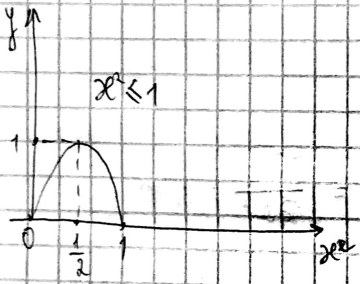
\includegraphics[width = 0.8\linewidth]{img_391}\\
$$
y(\text\ae ^2) = 4 \text\ae ^2 (1- \text\ae ^2)
$$
$$
max \{ |\lambda (\alpha)|; \alpha \in [0;2\pi] \} = 1, \text{если} \text\ae \leq 1 \Longrightarrow \text\ae = \frac{\tau}{h} \leq 1 - \text{условие устойчиости} 
$$
\end{document}
